\documentclass{standalone}
\usepackage{tikz}
\usetikzlibrary{shapes.geometric, arrows}
\usepackage[scaled]{helvet}
\usepackage[T1]{fontenc}
\renewcommand\familydefault{\sfdefault}


\tikzstyle{processnode} = [rectangle, rounded corners, 
minimum width=1.8cm, 
minimum height=1cm,
text width=1.8cm,
text centered, 
draw=black]

\tikzstyle{datanode} = [rectangle, thick,
fill=black!20,
minimum width=1.8cm, 
minimum height=1cm,
text width=1.8cm,
text centered, 
draw=black]

\tikzstyle{invisible} = [
minimum width=2cm, 
minimum height=1cm,
text width=2cm,
text centered]

\tikzstyle{io} = [trapezium, 
trapezium stretches=true, % A later addition
trapezium left angle=70, 
trapezium right angle=110, 
minimum width=3cm, 
minimum height=1cm, text centered, 
draw=black, fill=blue!30]

\tikzstyle{decision} = [diamond, 
minimum width=3cm, 
minimum height=1cm, 
text centered, 
draw=black, 
fill=green!30]

\tikzstyle{arrow} = [thick,->,>=stealth]
\begin{document}

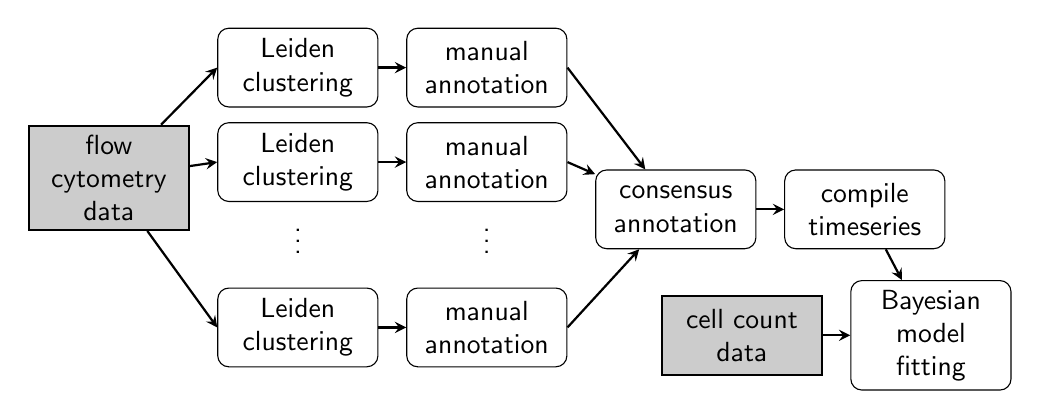
\begin{tikzpicture}[node distance = 1.2cm]
\def\xshift{1.2cm}

\node (start) [datanode] {flow\\ cytometry\\ data};

\node (clus1) [processnode, right of=start, xshift=\xshift, yshift=1.4cm] {Leiden clustering};
\node (clus2) [processnode, below of=clus1] {Leiden clustering};
\node (clus3) [invisible, below of=clus2, yshift=0.3cm] {$\vdots$};
\node (clus4) [processnode, below of=clus3] {Leiden clustering};

\node (ann1) [processnode, right of=clus1, xshift=\xshift] {manual\\ annotation};
\node (ann2) [processnode, below of=ann1] {manual\\ annotation};
\node (ann3) [invisible, below of=ann2, yshift=0.3cm] {$\vdots$};
\node (ann4) [processnode, below of=ann3] {manual\\ annotation};

\node (cons) [processnode, right of=ann1, xshift=\xshift, yshift=-1.8cm] {consensus annotation};

\node (time) [processnode, right of=cons, xshift=\xshift] {compile timeseries};
\node (count) [datanode, below of=cons, xshift=0.7*\xshift, yshift=-0.4cm] {cell count data};

\node (fit) [processnode, below of=time, xshift=0.7*\xshift, yshift=-0.4cm] {Bayesian model fitting};

\draw [arrow] (start) -- (clus1.west);
\draw [arrow] (start) -- (clus2.west);
\draw [arrow] (start) -- (clus4.west);

\draw [arrow] (clus1) -- (ann1);
\draw [arrow] (clus2) -- (ann2);
\draw [arrow] (clus4) -- (ann4);

\draw [arrow] (ann1.east) -- (cons);
\draw [arrow] (ann2.east) -- (cons);
\draw [arrow] (ann4.east) -- (cons);

\draw [arrow] (cons) -- (time);
\draw [arrow] (time) -- (fit);

\draw [arrow] (count) -- (fit);


\end{tikzpicture}
\end{document}